% \documentclass[12pt, twoside]{article}
\usepackage[letterpaper, margin=1in, headsep=0.2in]{geometry}
\setlength{\headheight}{0.6in}
%\usepackage[english]{babel}
\usepackage[utf8]{inputenc}
\usepackage{microtype}
\usepackage{amsmath}
\usepackage{amssymb}
%\usepackage{amsfonts}
\usepackage[nomessages]{fp} %\FPeval{\var-name}{2*sin(pi/6)}
\usepackage{siunitx} %units in math. eg 20\milli\meter
\usepackage{yhmath} % for arcs, overparenth command
\usepackage{tikz} %graphics
\usetikzlibrary{quotes, angles, arrows, arrows.meta}
\usepackage{graphicx} %consider setting \graphicspath{{images/}}
\usepackage{parskip} %no paragraph indent
\usepackage{enumitem}
\usepackage{multicol}
\usepackage{venndiagram}

\usepackage{fancyhdr}
\pagestyle{fancy}
\fancyhf{}
\renewcommand{\headrulewidth}{0pt} % disable the underline of the header
\raggedbottom
\hfuzz=2mm %suppresses overfull box warnings

\usepackage{hyperref}

\fancyhead[LE]{\thepage}
\fancyhead[RO]{\thepage \\ Name: \hspace{4cm} \,\\}
\fancyhead[LO]{BECA / Dr. Huson / Geometry\\*  Unit 3: Parallel lines and transversals\\* 17 October 2022}

\begin{document}

\subsubsection*{3.5 Proving the triangle sum theorem}
\begin{enumerate}
  \item Given isosceles $\triangle LMN$, $\overline{LM} \cong \overline{NM}$. If $m\angle L=5x-3$ and $m\angle N=7x-27$, find $m\angle M$.
  \begin{flushright}
  \begin{tikzpicture}[scale=0.8]
    %\draw [->, thick] (0,0)--(5,5);
    \draw [-, thick] (0,0) node[below]{$L$}--
      (2.5,3) node[above]{$M$}--
      (5,0) node[below]{$N$}--cycle;
  \end{tikzpicture}
  \end{flushright} \vspace{2cm}

\item The measures in degrees of the three angles of a triangle are $2x$, $\frac{2}{5}x$, and $\frac{1}{10}x$. Find the measures of the triangle's angles. \vspace{4cm}

\item Given two parallel lines, two transversals
\begin{multicols}{2}
  \begin{enumerate}
    \item Find $x$, $y$
    \item What relationship are you using? \\[0.5cm]
    (e.g. vertical angles, same-side exterior angles, alternate interior angles, etc.)
  \end{enumerate}
    \begin{tikzpicture}[scale=1.4]
    \draw [<->, thick] (4,2.25)--(7,2.25);
    \draw [<->, thick] (3.5,0)--(7,0);
    \draw [<->, thick] (4,-0.5)--(5.7,3);
    \draw [<->, thick] (6.5,-0.5)--(5,3);
    \node at (4.4,0.3) [right]{$69^\circ$};
    \node at (5.5,0.3) [right]{$86^\circ$};
    \node at (5.1,2.2) [below left]{$x$};
    \node at (5.5,2.2) [below right]{$y$};
  \end{tikzpicture}
\end{multicols}

\item A triangle has two angles measuring $x^\circ$ and $y^\circ$ respectively. Find the measure of the third angle as an expression of $x$ and $y$. \vspace{2cm}

\newpage
\item Given  $\triangle LMN$ with $m\angle L=2x+20$, $m\angle N=3x+5$, and $m\angle M=5x+5$. Find $x$.
  \begin{flushright}
  \begin{tikzpicture}[scale=0.8]
    %\draw [->, thick] (0,0)--(5,5);
    \draw [-, thick] (0,0) node[below]{$L$}--
      (2.5,3) node[above]{$M$}--
      (5,0) node[below]{$N$}--cycle;
  \end{tikzpicture}
  \end{flushright} \vspace{2cm}

\item The measures in degrees of the three angles of a triangle are $3x$, $\frac{1}{2}x+7$, and $5x-65$. Find $x$. \vspace{4cm}


\end{enumerate}
\end{document}